\chapter{Data Analysis}
In the analysis of experimental data, the primary goal is to extract a differential cross section for Coulomb dissociation of $^{17}$B as a function of relative energy between $^{15}$B and two neutrons. To achieve the goal, I will describe the procedure of identifying the secondary beam of ${}^{17}$B, and selecting events involving the fragment ${}^{15}$B and two neutrons. The flow of the data analysis is as follows.

\begin{center}
    \begin{enumerate}
        \item Select the event containing ${}^{17}$B beam by beam particle identification
        \item Select the event containing ${}^{15}$B fragment by fragment particle identification
        \item Select the event containing two neutrons by cross-talk analysis
        \item Extract the 2$n$ removal cross section of the ${}^{17}\text{B} \to {}^{15}\text{B} + 2n$ reaction
        \item Reconstruct invariant mass at target and obtain the relative energy spectrum 
    \end{enumerate}
\end{center}

\section{Secondary Beam Particle Identification}

The identification of the ${}^{17}$B secondary beam was performed using the TOF-$B\rho$-$\Delta E$ method. Time of Flight (TOF) is obtained from time difference between scintillator at F7 and F13, $B\rho$ is calculated from the beam passing $x$ position at F5, and $\Delta E$ is measured from ionization chamber ICB. $A/Z$ and $Z$ of the secondary beam is driven by the following equation.

\begin{align}
    &\beta_{\text{TOF}_{\text{F7-F13}}} = L(\text{F7-F13}) / ( {\text{TOF}}_{\text{F7-F13}} \times c )\\
    &\beta_{\text{F5}} = f(\text{TOF}_{\text{F7-F13}})\\
    &A/Z = \frac{c \times B\rho_{\text{F5}} \times \gamma_{\text{F5}} }{ m_u \times \beta_{\text{F5}}} \label{eq:az}\\
\end{align}
\begin{align}
    Z = \beta_{\text{F7-F13}} \sqrt{\Delta E_{\text{ICB}} \bigg\{ 0.307075 \cdot \Delta x \bigg(\frac{Z_{\text{P10}}}{A_{\text{P10}}}\bigg) \ln \bigg( \frac{2m_{e}c^{2}\beta_{\text{F7-F13}}^{2}\gamma_{\text{F7-F13}}^{2}}{I_{\text{P10}}} - \beta_{\text{F7-F13}}^{2}\bigg) \bigg\}^{-1} }
\end{align}
$L(\text{F7-F13})$ is a distance between F7 and F13 scintillator, $f(\text{TOF}_{\text{F7-F13}})$ is 2nd order polynomial function of TOF for fitting $\beta_{\text{F5}}$. $\Delta E_{\text{ICB}}$ is total energy loss at ICB and $Z_{\text{P10}}$, $A_{\text{P10}}$ and $I_{\text{P10}}$ are effective atomic number, effective mass number and mean excitation energy of P10 gas. $\Delta x$ is a travel distance in ICB. The detail of each steps are described in following.

\subsection{Time of Flight}
The Time of Flight (TOF) is measured using the time difference between two plastic scintillators. In the present analysis, from the timing at F7 plastic scintillator ($t_{\text{F7}}$) and the ones from SBT1,2 at F13 ($t_{\text{SBT1}}$, $t_{\text{SBT2}}$), the TOF$_{\text{F7}-\text{F13}}$ is obtained by following equation.
    \begin{align}
        \text{TOF}_{\text{F7-F13}} = \frac{t_{\text{SBT1}} + t_{\text{SBT2}}}{2} - t_{\text{F7}} + \Delta t_{offset}
    \end{align}
$\Delta t_{offset}$ is the offset used to correct for the difference between the actual measured $\text{TOF}_{\text{F7-F13}}$ and the calculated TOF value with the consideration of energy loss at the materials between F7 and F13. The calculated $\text{TOF}_{\text{F7-F13}}$ value is 192.34 ns, and the corresponding $\Delta t_{offset}$ value is 172.03 ns.

\subsection{Magnetic Rigidity}
Magnetic Rigidity $B\rho$ is derived by Beam Projection Chamber (BPC) located at F5 dispersive focal plane. The $x$ position of a beam passing through F5 is measured by BPC, and the $B\rho$ is calculated using the following equation.
    \begin{align}
        B\rho = (1+\frac{x}{D}) B\rho_{0} \label{eq:brho}
    \end{align}
with the rigidity of the central trajectory $B\rho_{0}$ is 8.780 Tm, and  momentum dispersion $D$ is 3300 mm/$\%$. 

\subsection{Energy Loss}
The energy loss $\Delta E$ is measured in the Ionize Chamber for Beam (ICB). The correlation between $\Delta E$ and $Z$ can be obtained according to the simplified Bethe-Bloch's energy loss formula as follows.
    \begin{align}
        \frac{\Delta E}{\Delta x} = 2\pi N_{a} r_{e}^{2} m_{e} c^{2} \rho_{\text{P10}} 
        \bigg( \frac{Z_{\text{P10}}}{A_{\text{P10}}} \bigg) \bigg( \frac{Z^{2}}{\beta^{2}} \bigg) 
        \left[ \ln \frac{2m_{e}c^{2}\beta^{2}\gamma^{2}}{I_{\text{P10}}} - \beta^{2}  \right]
    \end{align}
with
    \begin{align}
        2 \pi N_{a} r_{e}^{2} m_{e} c^{2} \rho_{\text{P10}} = 0.307075 \text{ MeV cm}^{2} \text{g}^{-1} 
    \end{align}
    \begin{adjustwidth}{1cm}{}
        $N_{a}$ : Avogadro's number = 6.022 $\times$ 10$^{23}$\\
        $r_{e}$ : classical electron radius = 2.817 $\times$ 10$^{-13}$ cm\\ 
        $m_{e}$ : electron mass = 0.511 MeV/c$^{2}$\\
        $\rho_{\text{P10}}$ : density of the P10 gas = 1.84 $\times$ 10$^{-3}$ g/cm$^{3}$\\
        $Z_{\text{P10}}$ : effective atomic number of the P10 gas\\
        $A_{\text{P10}}$ : effective mass number of the P10 gas\\
        $I_{\text{P10}}$ : mean excitation energy of the P10 gas\\ 
        $\beta$ = $v / c$ of the beam particle\\
        $\gamma$ = $1 / \sqrt{1-\beta^{2}}$
    \end{adjustwidth}
\vspace{3mm}
In this formula, the density effect correction $\delta$ or shell correction $C$ are skipped. Since the P10 gas is compound of 90$\%$ Ar and 10$\%$ CH$_{4}$, the mean excitation energy $I_{\text{P10}}$ is calculated based on \cite{LEO}. The travel distance in ICB, which is calculated as (total length of ICB) $\times$ (probability of each gas in P10) $\times$ (volume density).
\begin{align}
    \Delta x &= 51\times0.9\times0.0016608 + 51\times0.1\times0.000667 
\end{align}

\subsection{Beam Particle Identification}
Figure \ref{fig:Beam_PID} shows the histogram of the particle identification of the secondary beam, showing $Z$ versus $A/Z$. The total numbers of the secondary beam for each target is summarized in Table \ref{tab:Beam_PID}.

\begin{figure}[t]
    \centering
    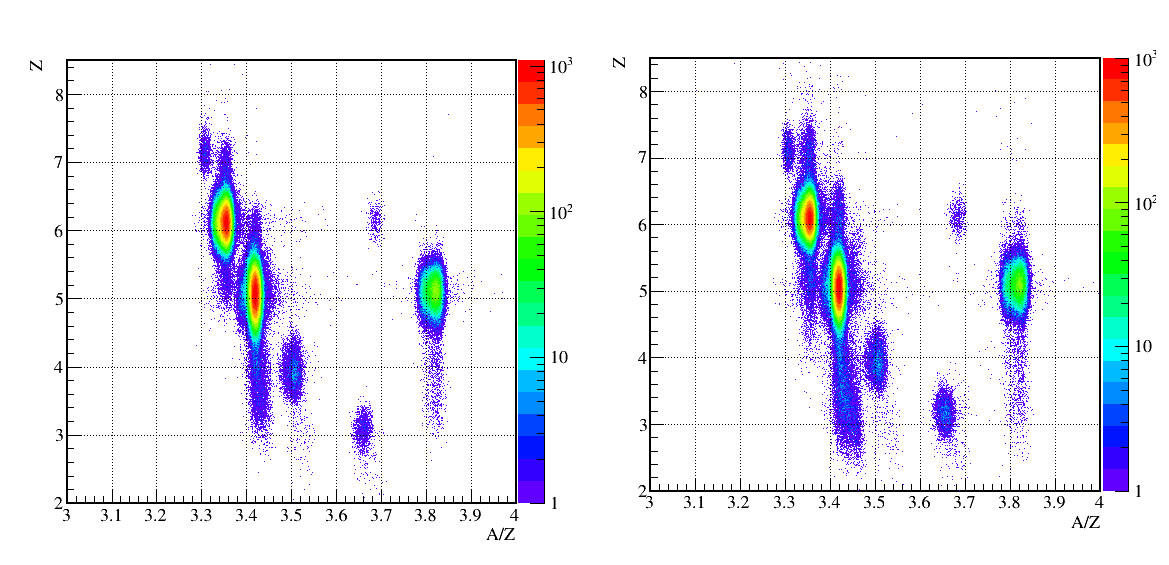
\includegraphics[width=0.8\textwidth]{chapter4/beampid.png}
    \caption[Secondary beam particle identification]{Beam particle identification of the secondary beam}
    \label{fig:Beam_PID}
\end{figure}

The gate condition for $^{17}$B is as follows.
\begin{itemize}
    \item DSB trigger 
    \item effective area of target $x <$ $\pm$ 35 mm and $y <$ $\pm$ 35 mm
    \item $4.40 < Z < 5.69$ and $3.4 < A/Z < 3.44$

\end{itemize}


\begin{table}[h]
    \centering
    \begin{tabular}{cccc}
        \hline
        Secondary Beam & Pb target & C target & Empty target\\             
        \hline
        ${}^{17}$B & 829586 & 756021 & 331445 \\
        ${}^{19}$B &  160905&  144243&  63033\\
        ${}^{20}$C &  1675080 & 1483113 & 510410 \\
        \hline
    \end{tabular}
    \caption{Statistic of secondary beam}
    \label{tab:Beam_PID}
\end{table}

%----------------------------------------------------------------------------------------------------

\section{Beam Profile at Target}

The beam profile at the target can be determined using the two drift chambers, BDC1 and BDC2, located upstream of the target. The incident position and angle at the target are obtained from the beam positions at BDC1 and BDC2.

\subsection{BDC Calibration}
The BDC drift chamber is designed for tracking the incident particle. Beam particle trajectory is obtained by following procedure.

\begin{enumerate}
    \item Obtain a drift time from TDC distribution.
    \item Extract a hit position of each layer from STC (Space to Time Conversion) function.
    \item Fit the trajectory with the linear function by the least-square method.
\end{enumerate}

\subsubsection{TDC (Time to Digital Converter) Distribution}
The timing information of the BDC is obtained by TDC (Time to Digital Converter). In figure \ref{fig:TDC_BDCs}, the TDC distribution of BDC1 and BDC2 are shown. Since we used common stop mode to take a TDC data in this experiment, the drift time is,
\begin{align}
    t_{drift} = t_{max} - t_{\text{TDC}}
\end{align}
where $t_{max}$ is the maximum TDC value. This TDC distribution is obtained from run 431 with $\pm$ 5mm slit at F5. 

\subsubsection{STC (Space to Time Conversion) Function}
The distance between hit position to an anode wire is given by space time conversion (STC) from the drift time. Assuming the uniform position distribution in each drift length cell as
\begin{align}
    \frac{dN}{dx} = const.  
\end{align}
The STC function is derived by integrating the TDC distribution as,
\begin{align}
    &\frac{dN}{dt} \cdot \frac{dt}{dx} = const.\\
    &dx = C \cdot \frac{dN}{dt} \cdot dt,\\
    &x(t) = C \cdot \int_{t_{0}}^{t} \frac{dN}{dt} dt \label{eq:stc}
\end{align}
where, C is normalization factor, $t_0$ is the minimum drift time and $t$ is the drift time from TDC distribution. 
The integration range of TDC for each BDC is shown in table \ref{tab:TDC_BDCs}. The upper and lower limit is determined by the TDC distribution. (Figure \ref{fig:TDC_BDCs}) 
\begin{table}[h]
    \centering
    \begin{tabular}{c|cc}
        \hline
        &Lower limit [ch]& Upper limit [ch]\\
        \hline
        BDC1&640&760\\
        BDC2&630&750\\        
        \hline
    \end{tabular}
    \caption[TDC integration ranges of BDCs]{TDC integration ranges of BDC1 and BDC2}
    \label{tab:TDC_BDCs}
\end{table}

\begin{figure}[h]
    \centering
    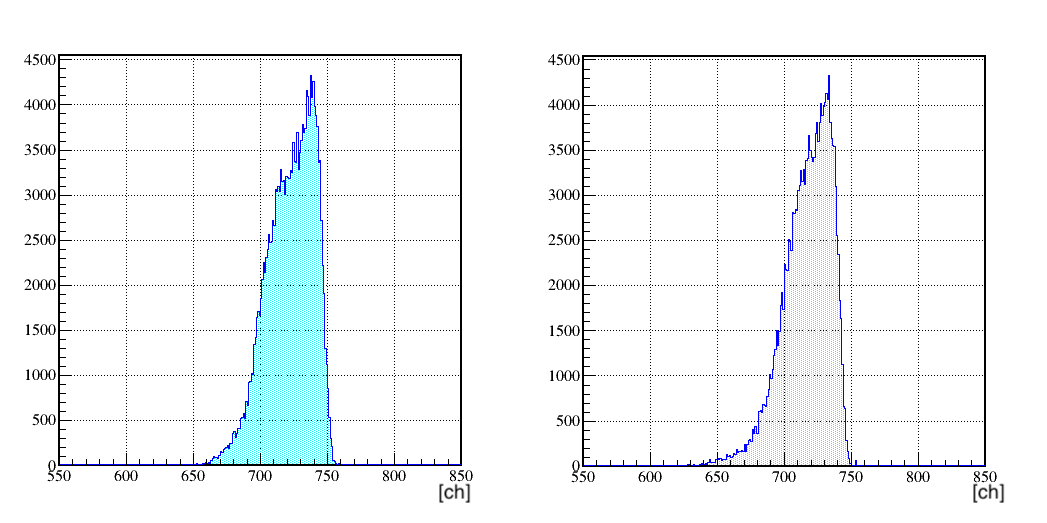
\includegraphics[width=14cm]{chapter4/BDCs_TDC.png}
    \caption[TDC Distribution of BDCs]{TDC Distribution of BDC1 (left) and BDC2 (right)}
    \label{fig:TDC_BDCs}
\end{figure}

\subsubsection{Linear fitting of trajectory}
After getting the STC function, the hit position of each layer is calculated from drift time as eq. (\ref{eq:stc}). Now we can get the trajectory of beam particle by fitting the hit position with linear function. When fitting the trajectory, the least-square method is used. The least-square method is the method of finding the best fit of a set of hit positions by minimizing the $\chi^2$ value. The $\chi^2$ value is defined as,
\begin{align}
    \chi^2 = \sum_{i=1}^{N} \frac{(x_{i} - f(x_{fit}))^2}{\sigma_{i}^2}
\end{align}
where, $x_{i}$ is the hit position of each layer, $f(x_{fit})$ is the position from fitting function, $\sigma_{i}$ is the position resolution of each layer.

\subsubsection{The resolution of BDCs}
After tracking the trajectory, the resolution of BDCs can be evaluated by the tracking residue distribution. The tracking residue $x_{residue}$ is defined as,

\begin{align}
    x_{residue} = x_{trac} - x_{drift}
\end{align}

where $x_{trac}$ is the calculated position from the trajectory and $x_{drift}$ is the hit position of each layer. The tracking residue distribution of BDC1 and BDC2 are shown in Figure \ref{fig:residue_bdcs}. The width of residue distribution for $x$ and $y$ direction are $\Delta x$ = 0.2605 mm, $\Delta y$ = 0.2632 mm respectively. From this, the position and angular resolution are calculated as described in the Appendix A. The result is described in table \ref{tab:resolution_bdcs}.

\begin{figure}
    \centering
    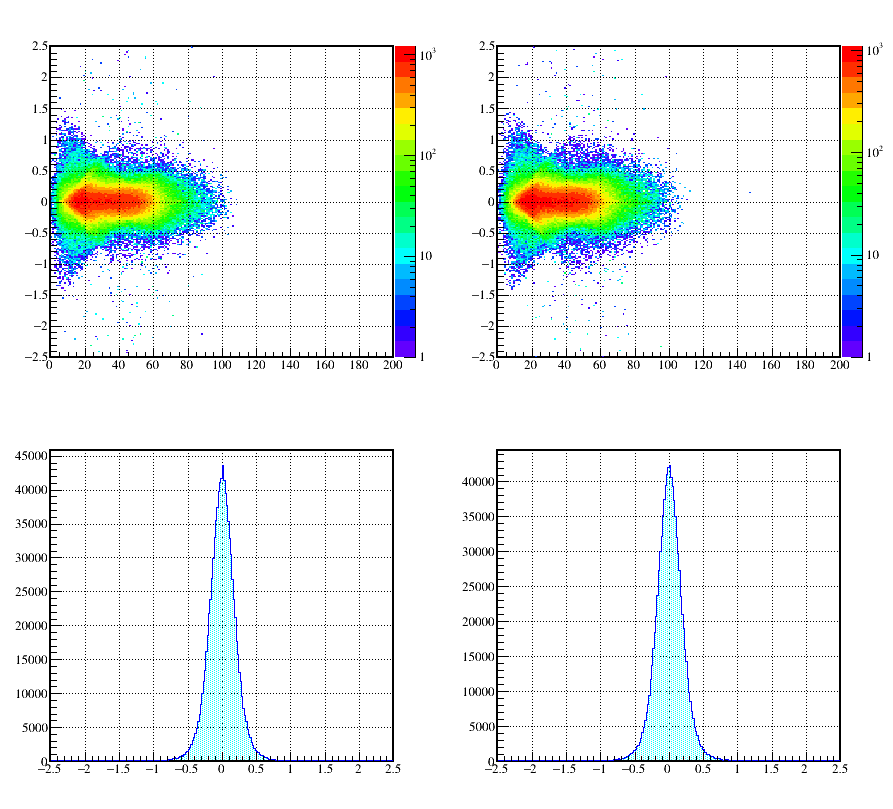
\includegraphics[width=12cm]{chapter4/BDC_residu.png}
    \caption[Tracking Residue Distribution of BDCs]{Tracking Residue Distribution of BDC1 (left) and BDC2 (right)}
    \label{fig:residue_bdcs}
\end{figure}

\begin{table}
    \centering
    \begin{tabular}{c|cc}
    \hline
     & $\sigma_x$ [mm] & $\sigma_y$ [mm]\\
    \hline
    BDC1 & 0.1340 & 0.1627 \\
    BDC2 & 0.1422 & 0.1743 \\
    \hline 
    \hline
    & $\sigma_a$ [rad] & $\sigma_b$ [rad]\\
    \hline
    BDC1 & 0.01316 & 0.01330 \\
    BDC2 & 0.01396 & 0.01424 \\
    \hline
    \end{tabular}
    \caption{Position and Angular Resolution of BDCs}
    \label{tab:resolution_bdcs}
\end{table}

\clearpage

\subsection{Beam Profile at Target}
The beam profile at the target is obtained by using the position information from BDCs. The position information ($x_{\text{tgt}}$, $y_{\text{tgt}}$) and angle information ($a_{\text{tgt}}$, $b_{\text{tgt}}$) at the target are obtained as,

\begin{align}
    x_{\text{tgt}} &= x_{\text{BDC1}} + \frac{(x_{\text{BDC2}} - x_{\text{BDC1}})}{L(\text{BDC1} - \text{BDC2})} \times L(\text{BDC1} - \text{tgt})\\
    y_{\text{tgt}} &= y_{\text{BDC1}} + \frac{(y_{\text{BDC2}} - y_{\text{BDC1}})}{L(\text{BDC1} - \text{BDC2})} \times L(\text{BDC1} - \text{tgt})\\
    a_{\text{tgt}} &= tan^{-1} \bigg( \frac{(x_{\text{BDC2}} - x_{\text{BDC1}})}{L(\text{BDC1} - \text{BDC2})} \bigg)\\
    b_{\text{tgt}} &= tan^{-1} \bigg( \frac{(y_{\text{BDC2}} - y_{\text{BDC1}})}{L(\text{BDC1} - \text{BDC2})} \bigg),
\end{align}
where the distance between BDCs is $L(\text{BDC1} - \text{BDC2}) = 999.32$mm, and the distance between BDC1 and the target is $L(\text{BDC1} - \text{tgt}) = 2017.13$mm. The beam profile at the target is shown in Figure \ref{fig:beam_profile_tgt}.
\begin{figure}[h]
    \centering
    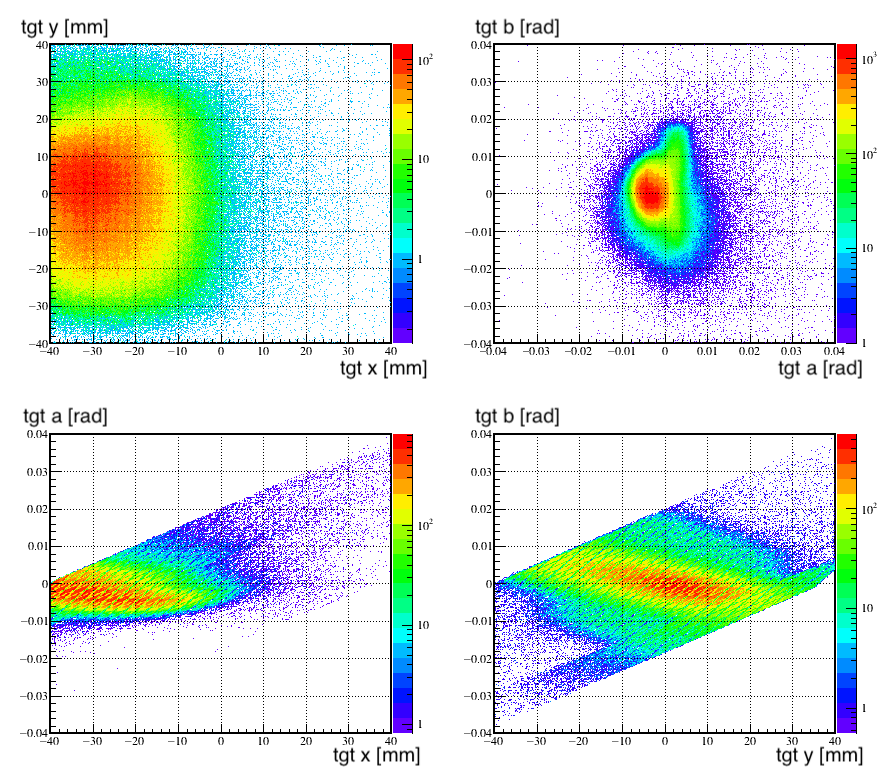
\includegraphics[width=10cm]{chapter4/target.png}
    \caption{${}^{17}$B Beam profile at target}
    \label{fig:beam_profile_tgt}
\end{figure}

\subsection{Position and Angular Resolution at Target}
\begin{align}
    \Delta \theta_x^{\text{tgt}} = \Delta \bigg( \frac{x_{\text{BDC2}} - x_{\text{BDC1}}}{L(\text{BDC2} - \text{BDC1})} \bigg) 
    = \frac{\sqrt{(\Delta x_{\text{BDC2}})^2 + (\Delta x_{\text{BDC1}})^2}}{999.32 \text{mm}} = 0.196 \text{mrad}\\
    \Delta \theta^{\text{tgt}}_y = \Delta \Big( \frac{y_{\text{BDC2}} - y_{\text{BDC1}}}{L(\text{BDC2} - \text{BDC1})} \Big) 
    = \frac{\sqrt{(\Delta y_{\text{BDC2}})^2 + (\Delta y_{\text{BDC1}})^2}}{999.32 \text{mm}} = 0.239 \text{mrad}
\end{align}
The position resolution at the target is
\begin{align}
    \Delta x_{\text{tgt}} = \sqrt{(\Delta x_{\text{BDC2}})^2 + (\Delta \theta_x^{\text{tgt}} \cdot L(\text{tgt} - \text{BDC2}))^2} = 0.24 \text{mm}\\ 
    \Delta y_{\text{tgt}} = \sqrt{(\Delta y_{\text{BDC2}})^2 + (\Delta \theta_y^{\text{tgt}} \cdot L(\text{tgt} - \text{BDC2}))^2} = 0.28 \text{mm}
\end{align}

\clearpage

\section{Charged Particle Identification}

Charged particles are identified using the TOF-B$\rho$-$\Delta$E method as same as the beam particle identification. Time of Flight is obtained from time difference between target and HODF, $B\rho$ is calculated from FDC1 and FDC2 positions and angles, and $Z$ is calculated by HOD $Q$ information. $A/Z$ and $Z$ is obtained by the following equation.

\begin{align}
    &\beta_{\text{frag}} = L(\text{tgt - HODF}) / ( {\text{TOF}}_{\text{tgt - HODF}} \times c )\\
    &A/Z = \frac{c \times B\rho \times \gamma_{\text{frag}}} { m_u \times \beta_{\text{frag}}}\\
    &Z = p_0 + p_1 (Q_{\text{HOD}} - p_2 \frac{1}{\beta^2})
\end{align}

$L$(tgt - HODF) is flight length from target to HODF. This is also calculated by a function of the positions and angles at FDC1 and FDC2 as the one for $B\rho$. The coefficient of $Z$ calculation $p_0, p_1, p_2$ are obtained by linear fitting of HOD $Q$ distribution. The detail of each steps will be described in following.

\subsection{FDC Calibration}
The tracking procedure of FDCs is same as BDC. The integration range of TDC for each FDC is shown in table \ref{tab:TDC_FDCs} And the TDC distribution for determining the upper and lower limit are shown in Figure \ref{fig:TDC_FDCs}. 
\begin{table}[h]
    \centering
    \begin{tabular}{c|cc}
        \hline
        &Lower limit [ch]&Upper limit [ch]\\
        \hline
        FDC1&1300&1600\\
        FDC2&500&1470\\        
        \hline
    \end{tabular}
    \caption[TDC integration range of FDCs]{TDC integration ranges of FDC1 and FDC2}
    \label{tab:TDC_FDCs}
\end{table}

\begin{figure}
    \centering
    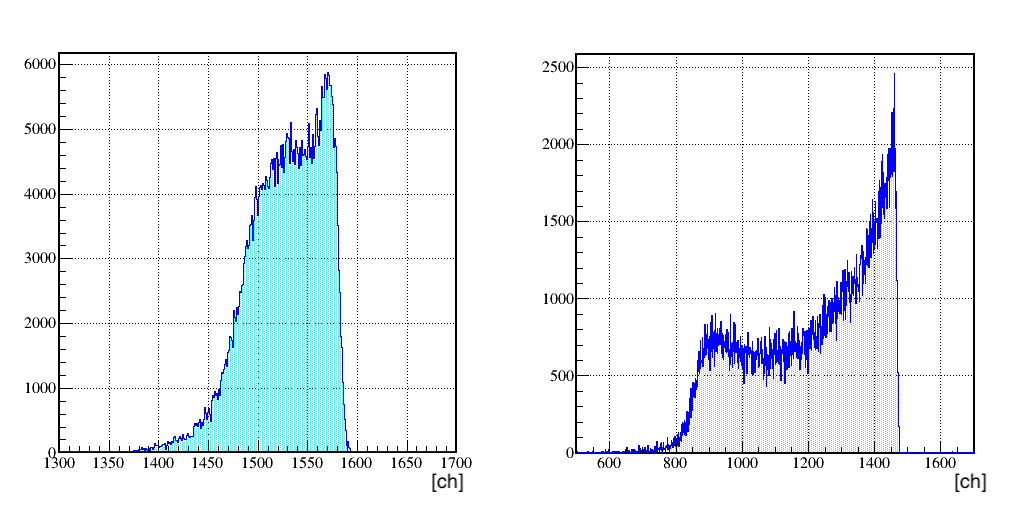
\includegraphics[width=14cm]{chapter4/FDCs_TDC.png}
    \caption[TDC Distribution of FDCs]{TDC Distribution of FDC1 (left) and FDC2 (right)}
    \label{fig:TDC_FDCs}
\end{figure}

\subsubsection{The resolution of FDCs}
The residue distributions of all plane of FDCs are shown in Figure \ref{fig:residue_fdcs}. From this, the position and angular resolution are calculated as described in the Appendix A. The result is described in table \ref{tab:resolution_fdcs}.

 \begin{figure}
    \centering
    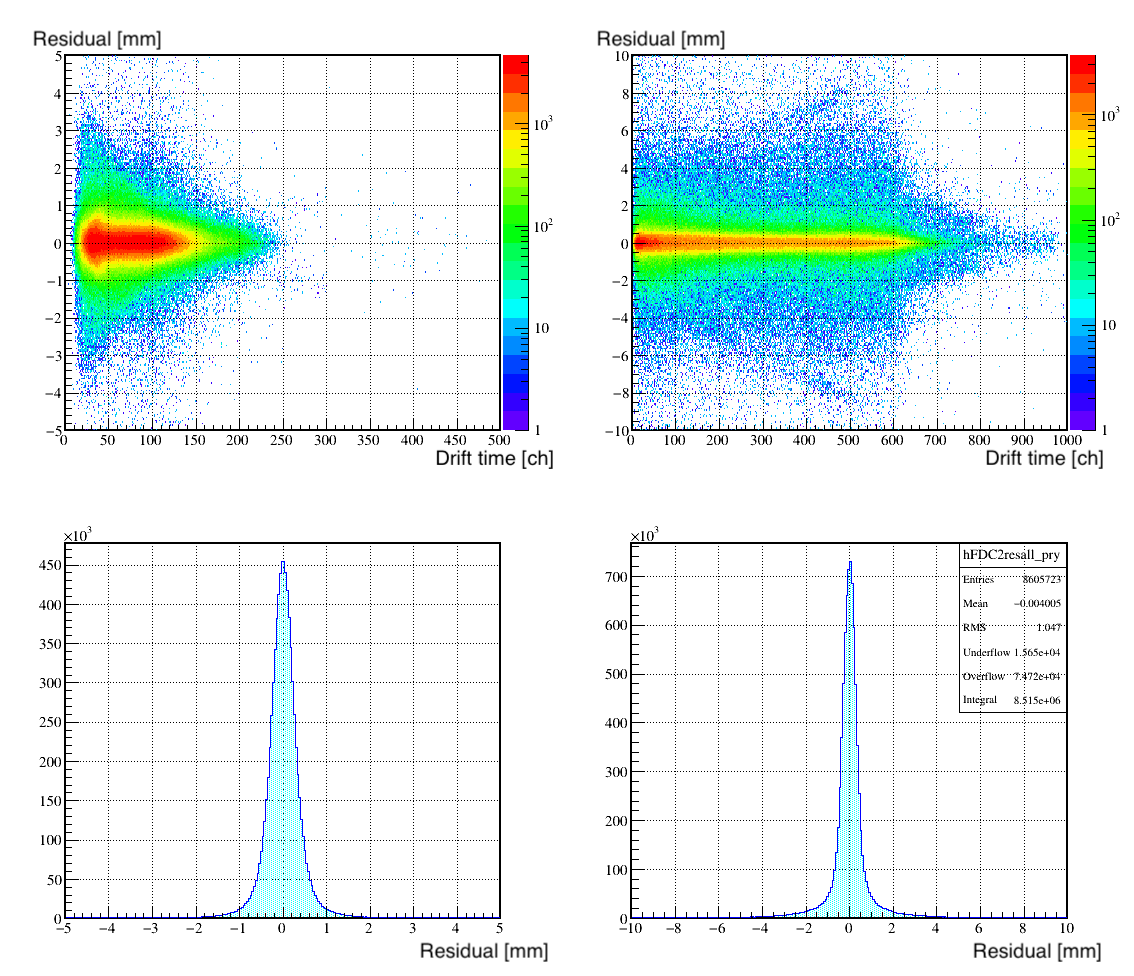
\includegraphics[width=12cm]{chapter4/FDC_residu.png}
    \caption[Tracking Residue Distribution of FDCs]{Tracking Residue Distribution of FDC1 (left) and FDC2 (right)}
    \label{fig:residue_fdcs}
\end{figure}

\begin{table}[h]
    \centering
    \begin{tabular}{c|cc}
        \hline
                &  $\Delta x_0$ [mm] & $\Delta y_0$ [mm]\\
            \hline
            FDC1 & 0.1239 & 0.2944 \\
            FDC2 &  0.1450 & 0.3443\\
            \hline
    \end{tabular}

    \begin{tabular}{c|cc}
    \hline
        & $\Delta a_0$ [rad] & $\Delta b_0$ [rad]\\
        \hline
        FDC1 & 0.00289 & 0.00948\\
        FDC2 & 0.00068 & 0.00224 \\
        \hline
    \end{tabular}
    \caption{Position and angular resolution of FDCs}
    \label{tab:resolution_fdcs}
\end{table}

\subsubsection{The efficiency of FDCs}
The efficiency of FDCs is evaluated by the tracking efficiency. The tracking efficiency is defined as the ratio of the number of events with a track at FDCs to the number of events with a hit at HODF. The definition of each efficiency can be written in following equation.
\begin{align}
\epsilon_{\text{FDC1}} = \frac{N (\text{FDC1} \cap \text{HODF})}{N (\text{HODF})}\\    
\epsilon_{\text{FDC2}} = \frac{N (\text{FDC2} \cap \text{HODF})}{N (\text{HODF})}
\end{align}
The efficiency of FDC1 and FDC2 of $^{15}$B fragment for lead target is 96.0\% and 99.9\% respectively. The efficiency of FDC1 and FDC2 for carbon target is 93.1\% and 99.9\% respectively. And the efficiency of FDC1 and FDC2 for empty target is 98.9\% and 99.9\% respectively.

\subsection{Magnetic Rigidity}
The Brho of the charged particle is calculated from the positions and angles obtained from FDC1 and FDC2. The $B\rho$ is calculated by the following equation.
\begin{align}
    B\rho &= f(x_{\text{FDC1}}, y_{\text{FDC1}}, a_{\text{FDC1}}, b_{\text{FDC1}}, x_{\text{FDC2}}, a_{\text{FDC2}})\\
    &= \sum_{i} c_{1,i} a_i + \sum_{i}\sum_{j} c_{2,ij} a_i a_j + \sum_{i}\sum_{j}\sum_{k} c_{3,ijk} a_i a_j a_k + \cdots \\
    &= c_{1,0} x_{\text{FDC1}} + c_{1,1} y_{\text{FDC1}} + \cdots + c_{2,00} x_{\text{FDC1}}^2 + c_{2,01} x_{\text{FDC1}} y_{\text{FDC1}} + \cdots + c_{3,000} x_{\text{FDC1}}^3 + \cdots
\end{align}
The function of B$\rho$ is extracted by using TMultiDimFit class in ROOT using a trajectory obtained from Geant4 simulation.

\subsection{Time of Flight and Energy Loss}
\subsubsection{Time of Flight}
Time of flight of charged particle is determined by the time difference between the HODF and the target. The time at target is determined by addition of the time at F13 and the time of flight from F13 to the target. The time of flight between F13 and the target is calculated with ${}^{17}$B beam with Energy loss calculation considered the material between F13 and the target. The time of flight between HODF and target is defined by the following equation.

\begin{align}
    t_{\text{tgt}} = t_{F13} + tof_{\text{F13-tgt}}
    tof_{\text{HODF-tgt}} = t_{\text{HODF}} - t_{\text{tgt}} + \Delta t_{offset}
\end{align}
where $t_{\text{HODF}}$ is timing information of HODF and $\Delta t_{offset}$ is obtained by Geant4 simulation as same as B$\rho$ analysis. The $\Delta t_{offset}$ is defined as 112.53 ns.

\subsubsection{Energy Loss}
In case of fragment, the energy loss is obtained from the light output information of HODF scintillator. From the Bethe-Bloch formula, we assumed that 
\begin{align}
    Z_{frag} \propto \beta_{frag} \sqrt{\Delta E} = \beta_{frag} \sqrt{Q_{\text{HODF}}}.
\end{align}
$\beta_{frag}$ is obtained from the time of flight information and $Q_{\text{HODF}}$ is the light output information of HODF. Because of the proportional relation between $Z_{frag}$ and $\sqrt{Q_{\text{HODF}}}$, it is difficult to identify the fragment particle by only energy loss information. So first we gate the fragment particle by ${}^{17}$B beam, and assumed that most of fragment came from ${}^{17}$B should be ${}^{17}$B itself. Then we can get coefficient for calculating the $Z$.

\subsection{Fragment Particle Identification}
The fragment particle identification is shown in figure \ref{fig:fragpid_all} and \ref{fig:fragpid_b17}. Figure \ref{fig:fragpid_all} is the fragment particle identification of all events. Figure \ref{fig:fragpid_b17} is the fragment particle identification only from ${}^{17}$B beam events. We selected the $^{15}$B events with $4.735 < Z < 5.275$ and $2.95 < A/Z < 3.07$ and $^{13}$B events with $4.735 < Z < 5.275$ and $2.58 < A/Z < 2.70$.
\begin{figure}
    \centering
    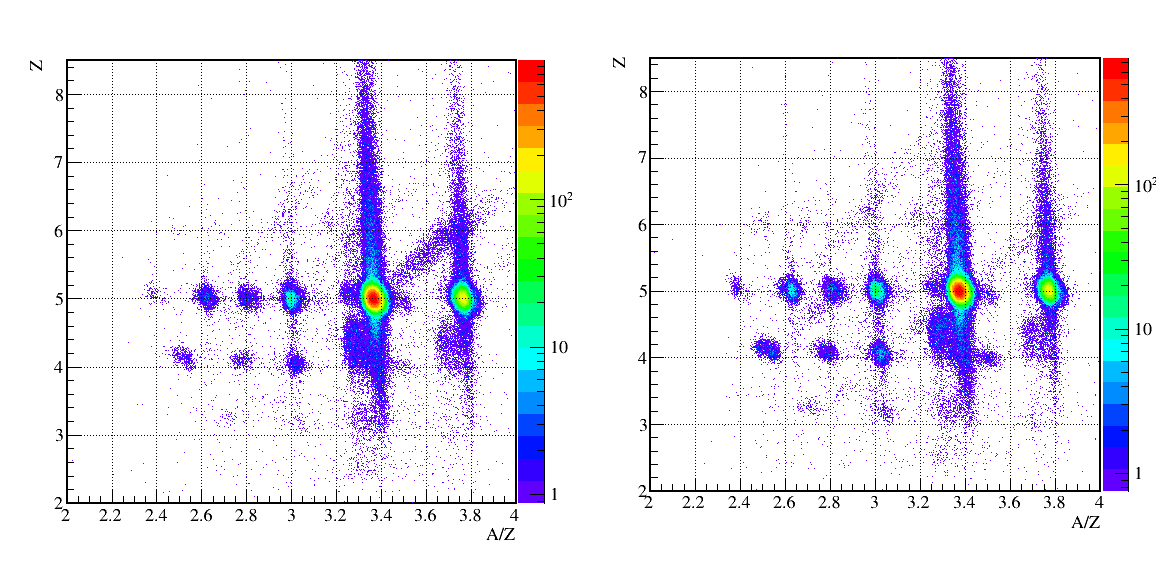
\includegraphics[width=\textwidth]{chapter4/fragpid_all.png}
    \caption[Fragment particle identification]{Fragment particle identification of all events at Pb target (left) and C target (right)}
    \label{fig:fragpid_all}
\end{figure}

\begin{figure}
    \centering
    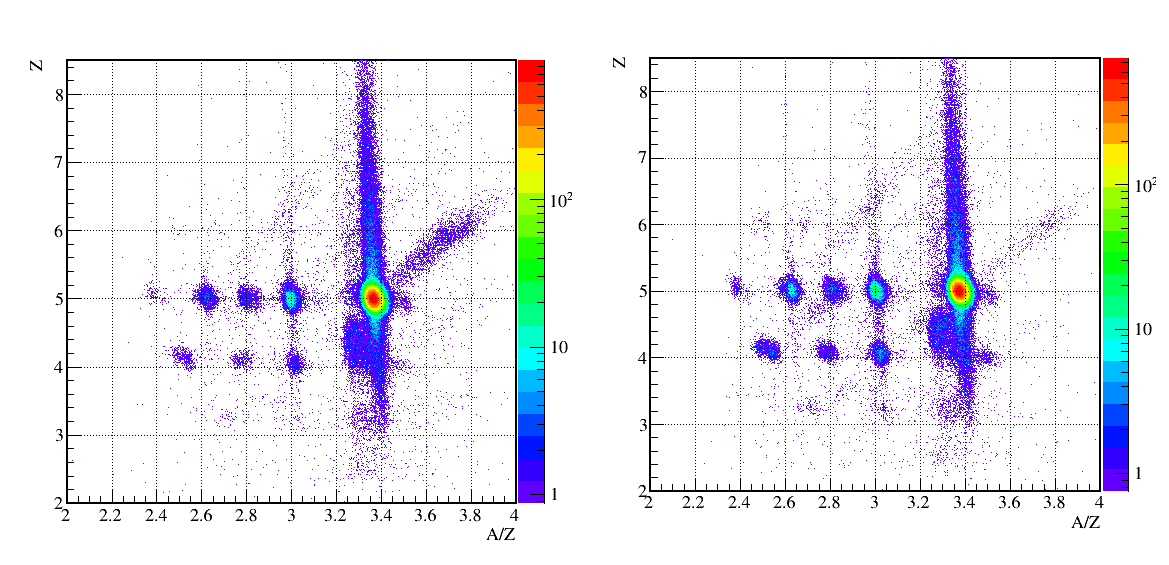
\includegraphics[width=\textwidth]{chapter4/fragpid_b17.png}
    \caption[Fragment particle identification from ${}^{17}$B beam]{Same as Figure\ref{fig:fragpid_all} but gated by ${}^{17}$B events at Pb target (left) and C target (right)}
    \label{fig:fragpid_b17}
\end{figure}

\clearpage

\section{Analysis of Neutrons}
In this experiment, neutrons emitted in the breakup reaction from the secondary beam ${}^{17}$B are detected by the NEBULA neutron detector array. A neutron is detected indirectly by recoiled proton which is mainly produced by H($n$,$n$) and ${}^{12}$C($n$,$np$) reaction in the plastic scintillator. The vector of neutron is determined as follows.
\begin{align}
    L &= | \vec{r}_{\text{tgt}} - \vec{r}_{n} | \\
    \beta_{n} &= L / (\text{TOF}_{\text{NEB-tgt}} \times c) \\
    P_{n} &= m_{n} \beta_{n} \gamma_{n} \\
    E_{n} &= m_{n} \gamma_{n} \\
    \vec{P_{n}} &= \frac{\vec{r_{n}} - \vec{r_{tgt}}}{L} P_{n}
\end{align}
where, $\vec{r}_{\text{tgt}}$ is the position of the target $\vec{r}_{\text{tgt}}$, $m_{n}$ is the neutron mass. In following section, the analysis of neutron events will be described.

\subsection {Selection of Real Neutron Events}
For the selection of neutron events, the events caused by charged particle and gamma ray should be rejected. In addition, in two neutron selection procedure, noise signals caused by multiple interaction of a single neutron, called cross-talk have to be eliminated. The selection of neutron events is performed in five steps as follows. 
\begin{enumerate}
    \item All events detected by the first VETO are considered to be charged particles and are rejected.
    \item Among the events detected by NEBULA, events with a light output Q of less than 6 MeVee are considered to be gamma rays and are rejected.
    \item Events whose TOF from the target to the first wall is less than 40 ns and whose TOF from the target to the second wall is less than 42 ns are considered to be non-neutron events with $\beta < 0.9$ and are rejected.
    \item (For the selection of two neutron events) For events detected at the second VETO, detections in which the two fastest neutron events incident on the second NEUT wall are dr(xy) $<$ 500mm and 1ns $<$ dt $<$ 5ns are considered to be cluster scattering events from second VETO and the second event is rejected.
    \item (For the selection of two neutron events) Cross-talk events are rejected.
\end{enumerate}
After these rejection procedure, we choose the first and second fastest event as a neutron event. In following section, the three step of cross-talk rejection procedure will be described.

\subsection{Cross-talk Rejection}
The conditions of the cross-talk rejection are determined based on a Geant4 simulation. To reject the cross-talk events, ${}^{16}\text{B} \to {}^{15}\text{B}+n$ simulation is performed, thereby replicating cases where all two-neutron events are due to cross-talk. The beam $^{16}$B is reconstructed based on the $^{17}$B beam information at target (Figure \ref{fig:beam_profile_tgt}). The details of the simulation are shown in Table \ref{tab:cross-talk_sim}.

\begin{table}
    \centering
    \begin{tabular}[h]{c|c}
        \hline 
        Reaction & ${}^{16}\text{B} \to {}^{15}\text{B}+n$ \\
        Beam energy & Reconstructed from $^{17}$B beam profile\\
        Relative energy & 0 - 10 MeV (Uniformly generated)\\
        Position distribution & Reconstructed from ${}^{17}$B beam profile\\
        Angular distribution & Reconstructed from ${}^{17}$B beam profile \\
        \hline
    \end{tabular}
    \caption{The Geant4 simulation condition for cross-talk rejection}
    \label{tab:cross-talk_sim}
\end{table}

\subsubsection{Clustering event}
The clustering event means the two events which are detected in very close distance in very small time interval. It means the second event is likely to be a recoil proton from the first event. The clustering event is rejected by the following condition.

\begin{figure}[h]
    \centering
    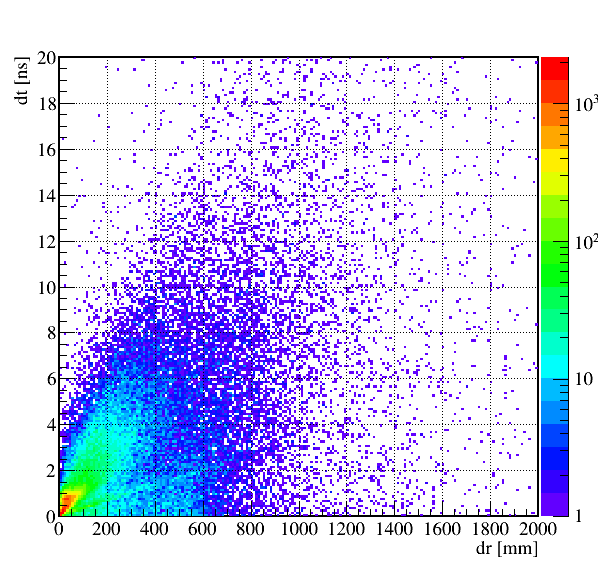
\includegraphics[width=8cm]{chapter4/drdt.png}
    \caption{Cross-talk simulation result of clustering event}
    \label{fig:clustering}
\end{figure}

\begin{align}
    \bigg( \frac{dr-dr_0}{3\sigma_{dr}} \bigg)^2 + \bigg( \frac{dt-dt_0}{3\sigma_{dt}} \bigg)^2 < 1 
\end{align}
where $dr$ and $dt$ are the position and time difference between two events. And $dr_0$ and $dt_0$, $\sigma_{dr}$ and $\sigma_{dt}$ mean the central values and the standard deviations of the distribution of $dr$ and $dt$ for the clustering events. The $dr_0$ and $dt_0$ are 98.35 mm and 0.65 ns, and $\sigma_{dr}$ and $\sigma_{dt}$ are 71.07 mm and 0.40 ns. 

\subsubsection{same wall event}
Figure\ref{fig:samewall} shows the cross-talk simulation result of same wall event. The right figure shows the distribution of light output of second event $Q_2$ with the function of relative velocity $\beta_{01}/\beta_{12}$ and the left one shows the distribution of $Q_2$ with $1/\beta_{12}$. After the selection of two neutron events, each event is tagged by the hit order. The light output is tagged as $Q_1$ and the one of second event is tagged as $Q_2$. The relative velocity between two events is defined as $\beta_{01}/\beta_{12}$ where $\beta_{01}$ represents the velocity between first hit and the target and $\beta_{12}$ represents the velocity between first and second hit. The cross-talk rejection condition of same wall event is defined as follows.
\begin{align}
    \frac{\beta_{01}}{\beta_{12}} > 1 \qquad \text{or} \qquad  \frac{\beta_{01}}{\beta_{12}} < -1.5
\end{align}

If the $\beta_{01}/\beta_{12}$ $>$ 1, it means the second event is slower than the first event and it is considered to be a cross-talk event caused by the scattered neutron from the first event. If the $\beta_{01}/\beta_{12}$ $<$ 0, it means the $z$ position of the second event is smaller than the first event. In this case, the cross-talk event can happen by the back scattering of the neutron from the first event. The condition of $\beta_{01}/\beta_{12}$ $<$ -1.5 is enough to reject this cross-talk event.
Another cross-talk rejection condition is determined by the $\gamma$ ray rejection. Considering that the $\gamma$ ray events distribute in the region of $1/\beta_{12} \sim \pm1$, the $\gamma$ ray rejection condition is defined as follows.
\begin{align}
    \bigg|\frac{1}{|\beta_{12}|} - 1\bigg| < 3\sigma_\gamma
\end{align}
The events in this region with the light output of second event $Q_2$ less than 20 MeVee are considered to be $\gamma$ ray events. The $\sigma_\gamma$ is the standard deviation of the distribution of $1/|\beta_{12}|$ for the $\gamma$ ray events. The $\sigma_\gamma$ is 0.1. 
\begin{figure}[h]
    \centering
    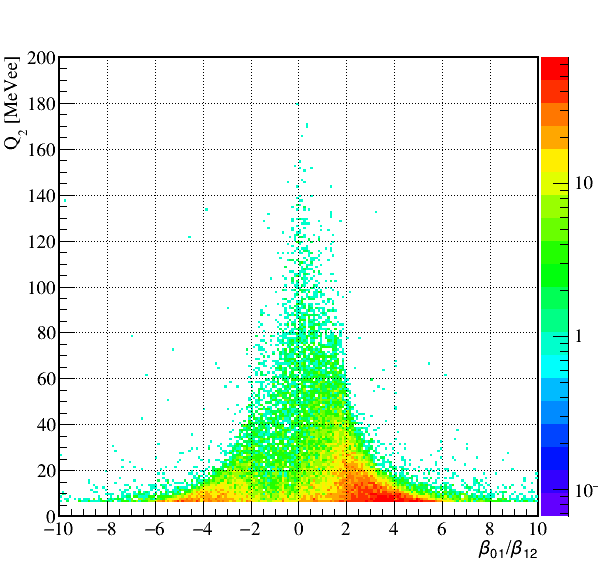
\includegraphics[width=0.4\textwidth]{chapter4/same1.png}\hspace{0.5cm}
    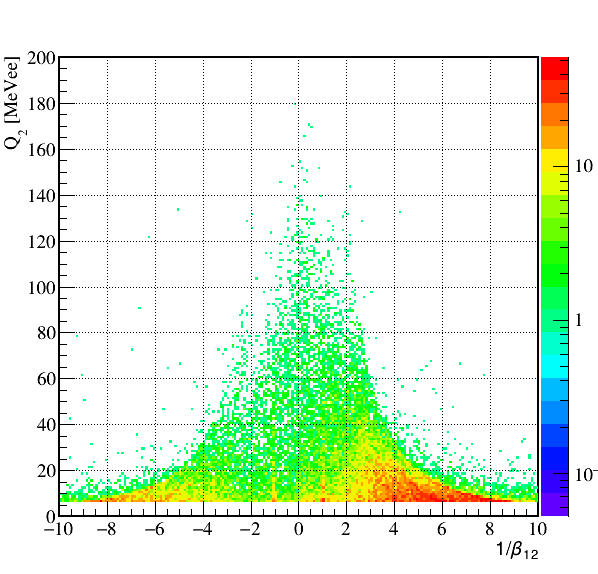
\includegraphics[width=0.4\textwidth]{chapter4/same2.png}
    \caption{Cross-talk simulation result of same wall event}
    \label{fig:samewall}
\end{figure}

\subsubsection{different wall event}
Figure \ref{fig:differentwall} shows the cross-talk simulation result of different wall event. The right figure shows the distribution of light output of second event $Q_1$ with the function of relative velocity $\beta_{01}/\beta_{12}$ and the left one shows the distribution of $Q_2$ with $1/\beta_{12}$. The cross-talk rejection condition of different wall event is similar to the same wall event, but in this case, $Q_1$ is used for the cross-talk rejection with the relative velocity. The cross-talk rejection condition of different wall event is defined as follows. 
\begin{align}
    \frac{\beta_{01}}{\beta_{12}} > 1 \qquad \text{or} \qquad  \frac{\beta_{01}}{\beta_{12}} < -1.5
\end{align}
And the $\gamma$ ray rejection is also performed using the distribution of $Q_2$ with $1/\beta_{12}$. The rejection condition is also defined as follows.
\begin{align}
    \bigg|\frac{1}{|\beta_{12}|} - 1\bigg| < 3\sigma_\gamma
\end{align}
The $\sigma_\gamma$ for different wall is 0.1.

\begin{figure}
    \centering
    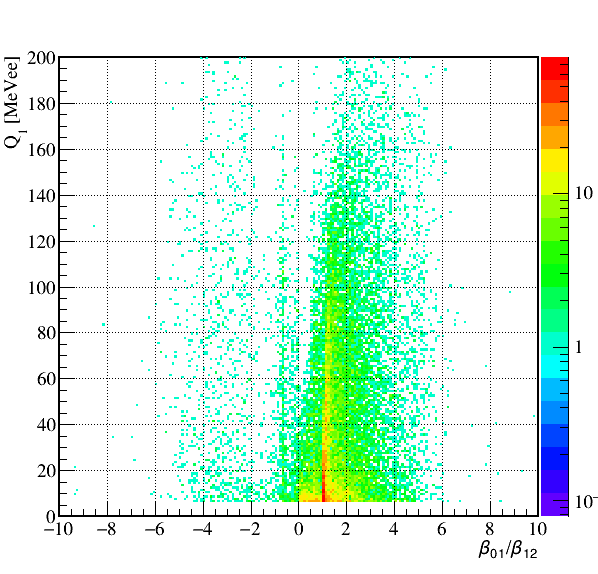
\includegraphics[width=0.4\textwidth]{chapter4/diff1.png}\hspace{0.5cm}
    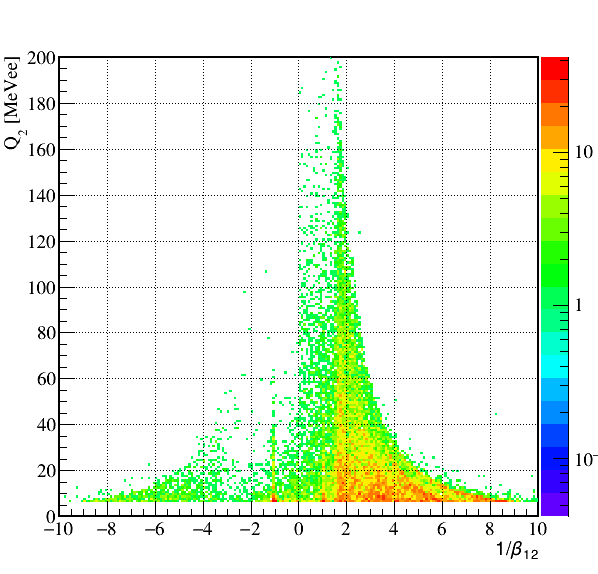
\includegraphics[width=0.4\textwidth]{chapter4/diff2.png}
    \caption{Cross-talk simulation result for different wall event}
    \label{fig:differentwall}
\end{figure}

\subsection{Cross-talk Residual Rate}
Even though we performed the cross talk rejection, there probably be residual of cross talk. For each cross talk step, we evaluated the residual rate of cross talk. Each step is as follows.
\begin{itemize}
    \item (a) no rejection
    \item (b) clustering rejection
    \item (c) clustering rejection + same wall rejection
    \item (d) clustering rejection + same wall rejection + gamma rejection
\end{itemize}
The residual rate of cross talk is given by the following equation.
\begin{align}
    R = \frac{N_{M>2}}{N_{M>1}}
\end{align}
The multiplicity $M>1$ event is 225385, $M>2$ event of each step and residual rate $R$ are written in Table \ref{cross-talk_residue}. The residual rates of same and different wall cross-talk are 2.4$\%$ and 0.9$\%$ respectively, when the all cross-talk rejection conditions are performed.
\begin{table}[h]
    \centering
    \begin{tabular}[h]{c|c|c|c}
        \hline
        Condition & same wall event (R) & different wall event (R) & all wall event (R)\\
        \hline
        (a) & 89721 (39.8$\%$) & 10123 (4.5$\%$) & 99844 (44.3$\%$) \\
        (b) & 29032 (12.9$\%$) & 16848 (7.5$\%$) & 45880 (20.4$\%$)\\
        (c) & 6274 (2.8)$\%$) & 2791 (1.2$\%$)& 9065 (4.0$\%$)\\
        (d) & 5352 (2.4$\%$)& 2089 (0.9$\%$)& 7441 (3.3$\%$)\\
        \hline
    \end{tabular}
    \caption{The cross talk residual rate evaluation}
    \label{cross-talk_residue}
\end{table}

\section{Acceptance and Efficiency Correction}
For evaluating the two-neutron detection efficiency and acceptance, the simulation is performed by Geant4. The information of simulation is as follows. The recoil effect at the reaction point is not considered in the simulation. The simulation condition is in the Table \ref{tab:2n_sim}.
\begin{table}[h]
    \centering
    \begin{tabular}[h]{c|c}
        \hline
        Physics Model & Phase Space Decay \\
        Reaction & ${}^{17}\text{B} \to {}^{15}\text{B} + 2n$\\
        Beam Energy & Reconstructed from $^{17}$B beam profile\\
        Relative Energy & 1-10 MeV (Uniformly generated)\\
        Scattering Angle & 0-30 mrad (Uniformly generated)\\
        \hline
    \end{tabular}
    \caption{The Geant4 simulation condition for two-neutron detection efficiency and acceptance}
    \label{tab:2n_sim}
\end{table}

The results of acceptance simulation for same and different wall are shown in figure \ref{fig:acc_same_diff}. $x$ axis is relative energy $E_{rel}$ between $^{15}$B and two neutrons, $y$ axis is scattering angle $\theta_{scat}$ in laboratory coordinate and $z$ axis is the detection efficiency. The acceptance of same wall in small $E_{rel}$ less than 0.5 MeV is very small because of the clustering cross-talk cut. The result of two-neutron detection efficiency curve for relative energy $E_{rel}$ is shown in figure \ref{fig:eff}. The blue line shows the same wall efficiency and the red line shows the different wall efficiency. The black line is the sum of the same and different wall efficiency. 
\begin{figure}[h]
    \centering
    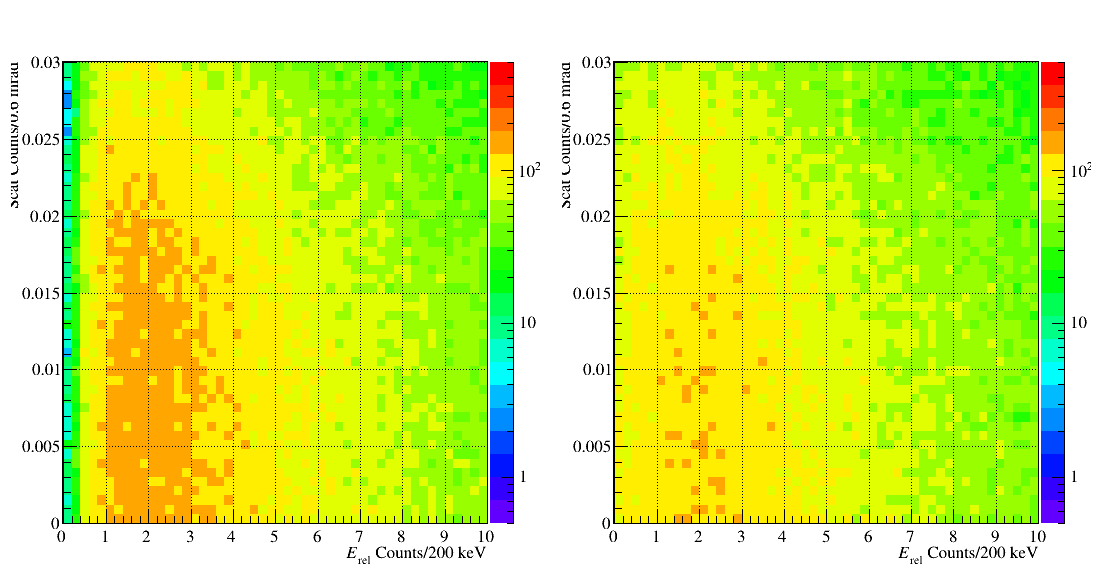
\includegraphics[width=\textwidth]{chapter4/acc_same_diff.png}
    \caption[$2n$ Acceptance for $E_{rel}$ and $\theta_{scat}$]{$2n$ Acceptance for same wall (left) and different wall (right)}
    \label{fig:acc_same_diff}
\end{figure}

\begin{figure}
    \centering
    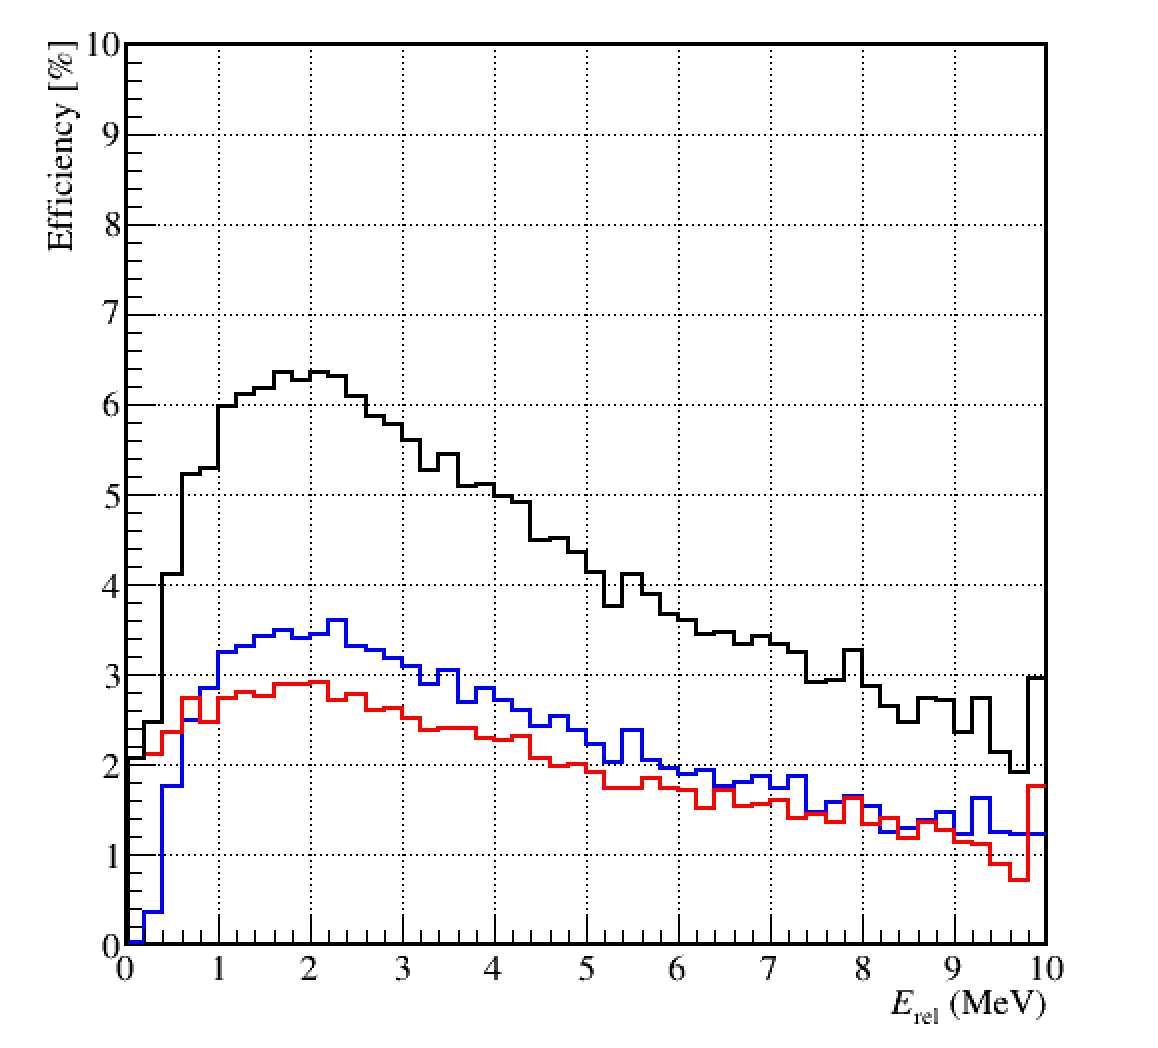
\includegraphics[width=10cm]{chapter4/Eff_curve.png}
    \caption[$2n$ detection efficiency for same wall and diff wall]{$2n$ Efficiency for same wall (left) and different wall (right)}
    \label{fig:eff}
\end{figure}

\clearpage
\section{Relative Energy Spectrum}
The relative energy $E_{rel}$ spectrum are reconstructed for the events where $^{15}$B and neutron(s) are detected. Figure \ref{fig:rel_energy_fnn} shows the relative energy spectrum of $^{15}$B and two neutrons. The relative energy spectrum of $^{15}$B and one neutron is shown in Figure \ref{fig:rel_energy_fn}. In the figures, the blue lines are the relative energy from the Pb or C target runs and the red lines are the one from empty target which is normalized with the number of events. The empty target runs will be subtracted as a background component. 
The differential cross section is calculated from the relative energy spectrum as follows.
\begin{align}
    \frac{d\sigma}{dE_{rel}} = \frac{1}{N_t} \cdot \frac{N_{i}}{N_{beam}} \cdot \frac{\text{LT}(\text{DSB})}{\text{LT}(\text{B} \cap \text{N})} \frac{1}{\epsilon_{\text{FDC1}} \epsilon_{\text{FDC2}} \epsilon_{acc} \epsilon_{eff}},
\end{align}
where $N_t$ is the number of target nucleons, $N_{i}$ is the number of events in the $i$-th bin, $N_{beam}$ is the number of beam particles, $\text{LT}(\text{DSB})$ and $\text{LT}(\text{B} \cap \text{N})$ are the live time of DSB and B $\cap$ N trigger respectively, $\epsilon_{\text{FDC1}}$ and $\epsilon_{\text{FDC2}}$ are the efficiency of FDC1 and FDC2, $\epsilon_{acc}$ is the acceptance and $\epsilon_{eff}$ is the efficiency of two-neutron detection. The differential cross section of $^{15}$B and two neutrons and $^{15}$B and one neutron are shown in Figure \ref{fig:sigma_fnn} and \ref{fig:sigma_fn}. 

\clearpage
\begin{figure}
    \centering
    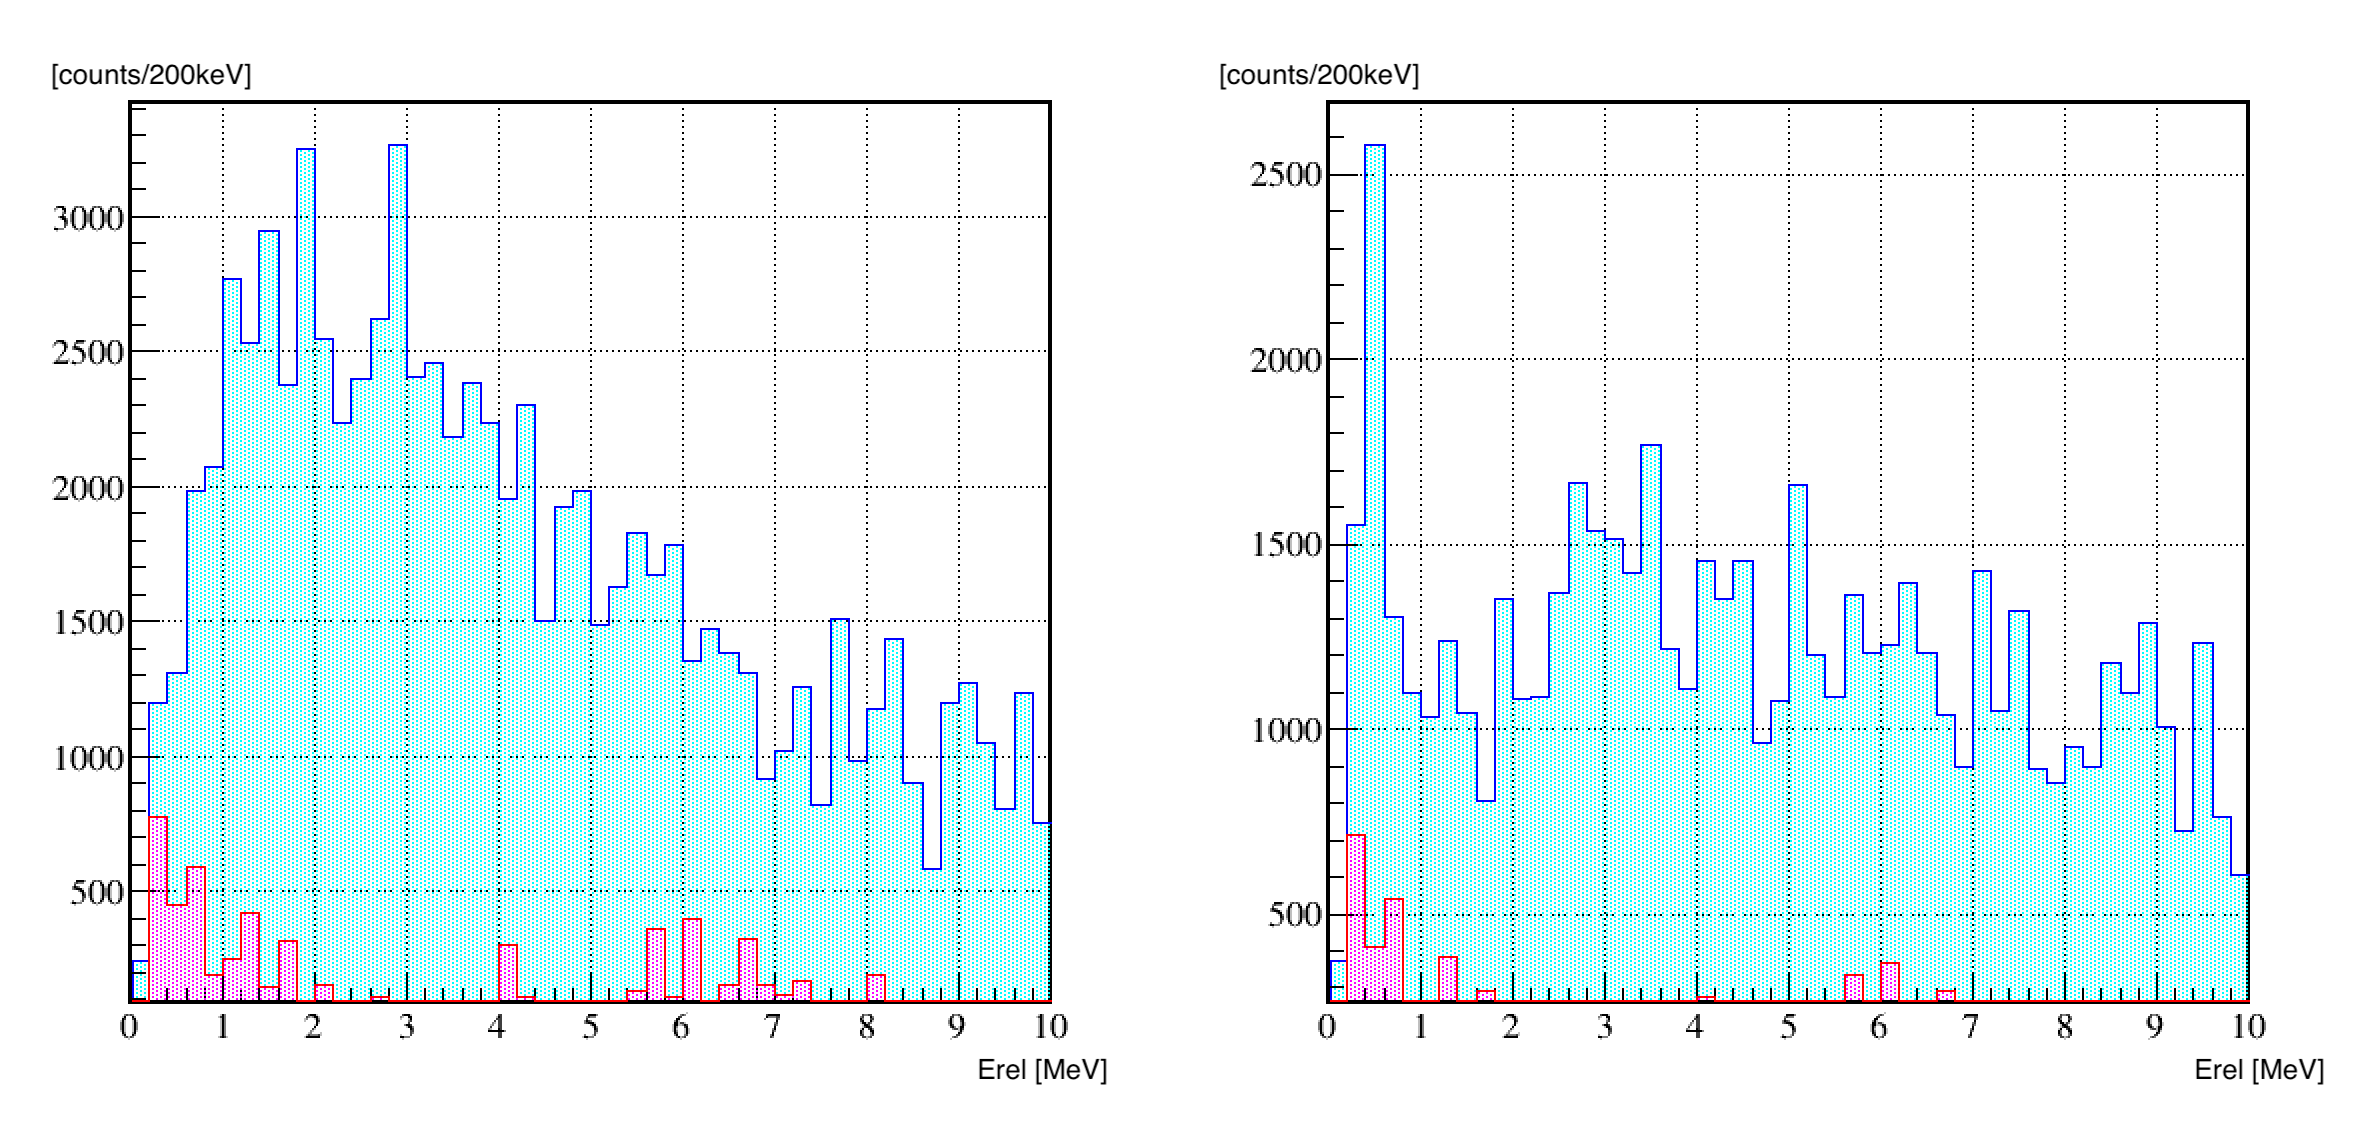
\includegraphics[width=\textwidth]{chapter4/fnn.png}
    \caption{Relative Energy Spectrum of ${}^{15}\text{B} + n + n$ at Pb target (left) and C target (right)}
    \label{fig:rel_energy_fnn}
\end{figure}

\begin{figure}
    \centering
    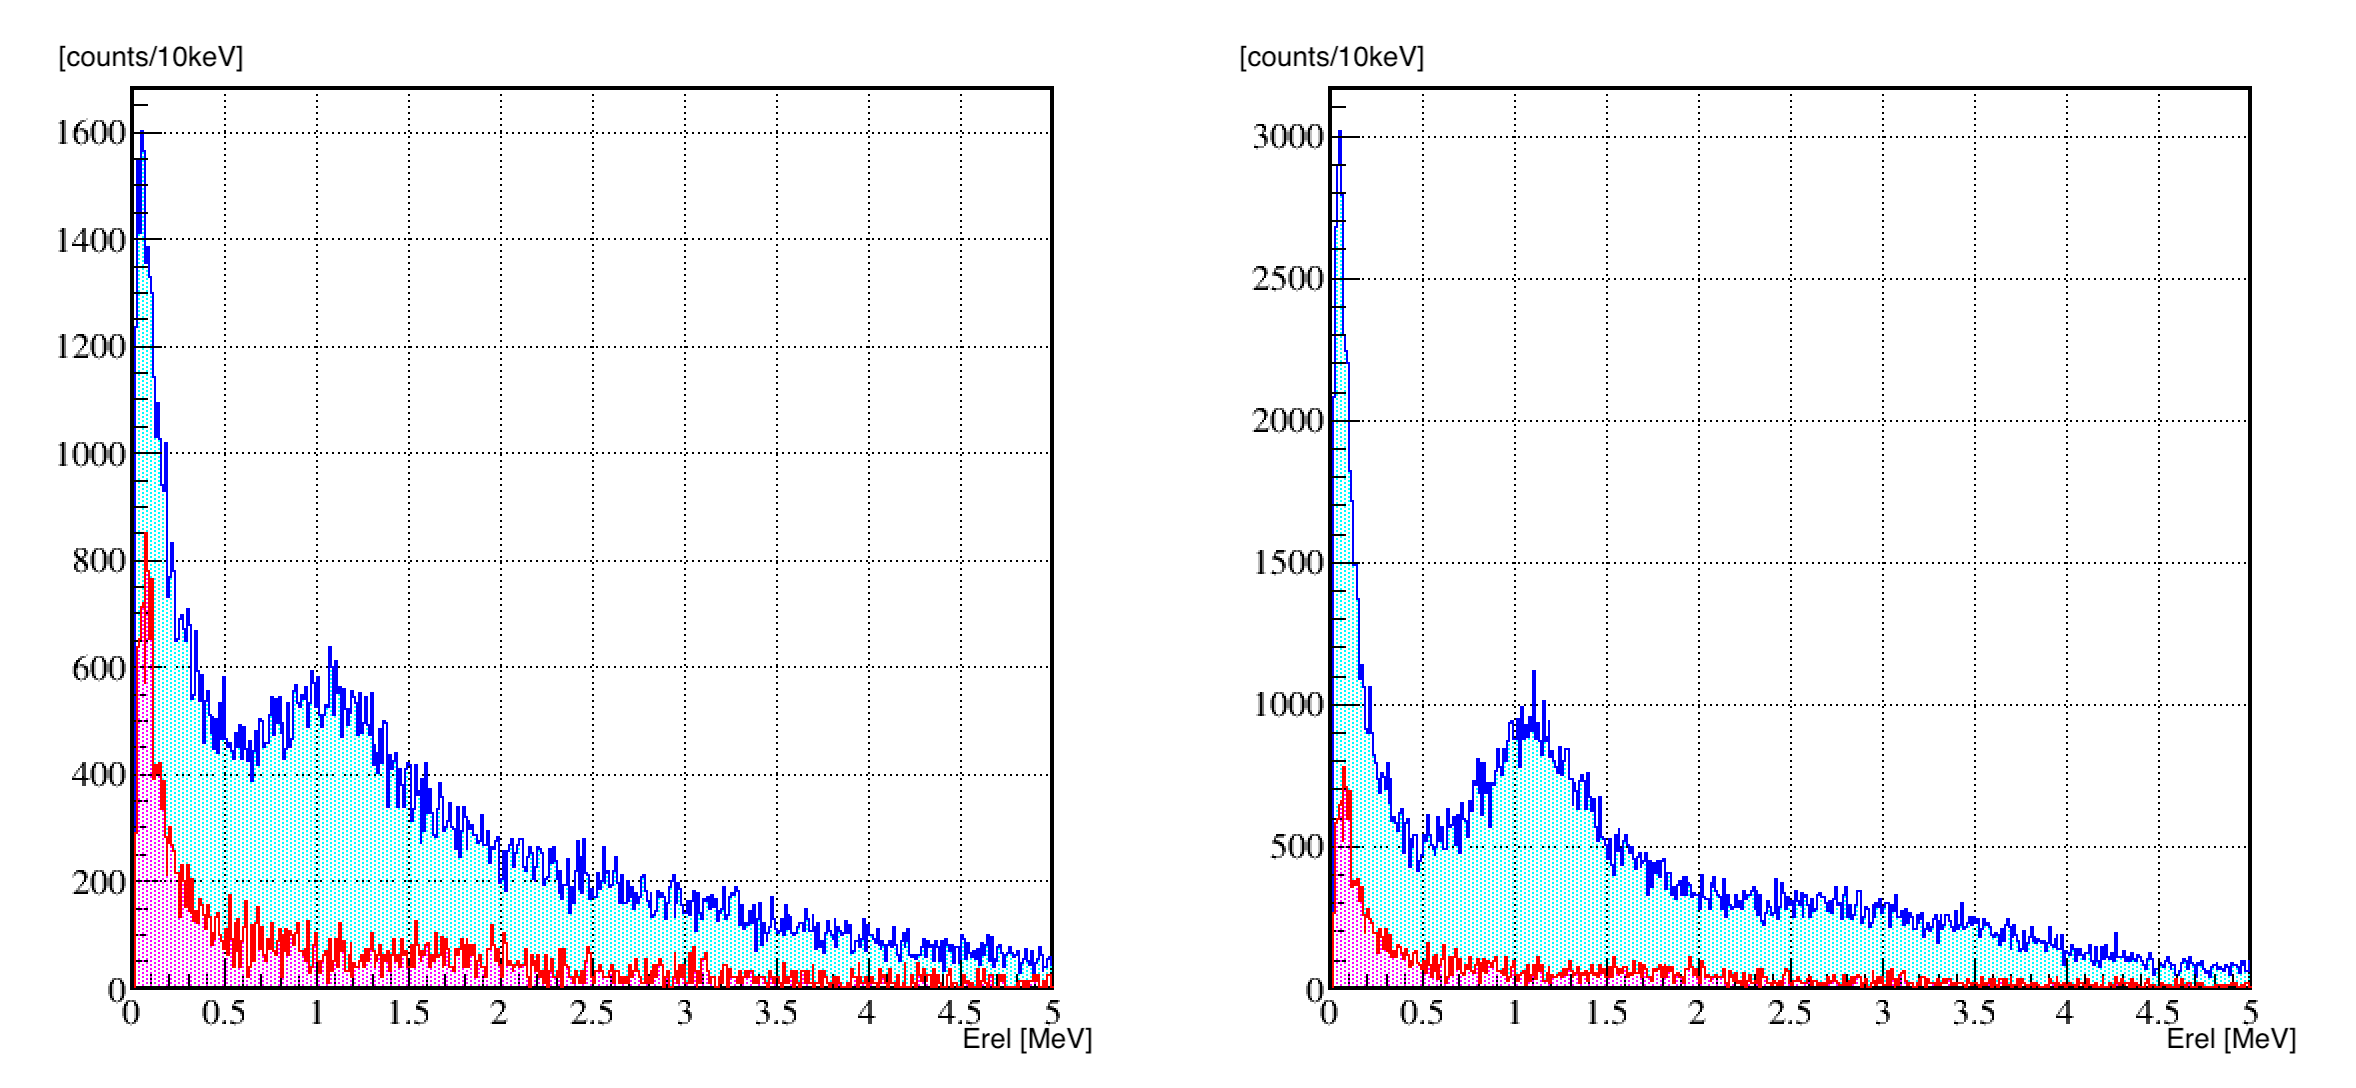
\includegraphics[width=\textwidth]{chapter4/fn.png}
    \caption{Relative Energy Spectrum of ${}^{15}\text{B} + n$ at Pb target (left) and C target (right)}
    \label{fig:rel_energy_fn}
\end{figure}

\clearpage
\begin{figure}
    \centering
    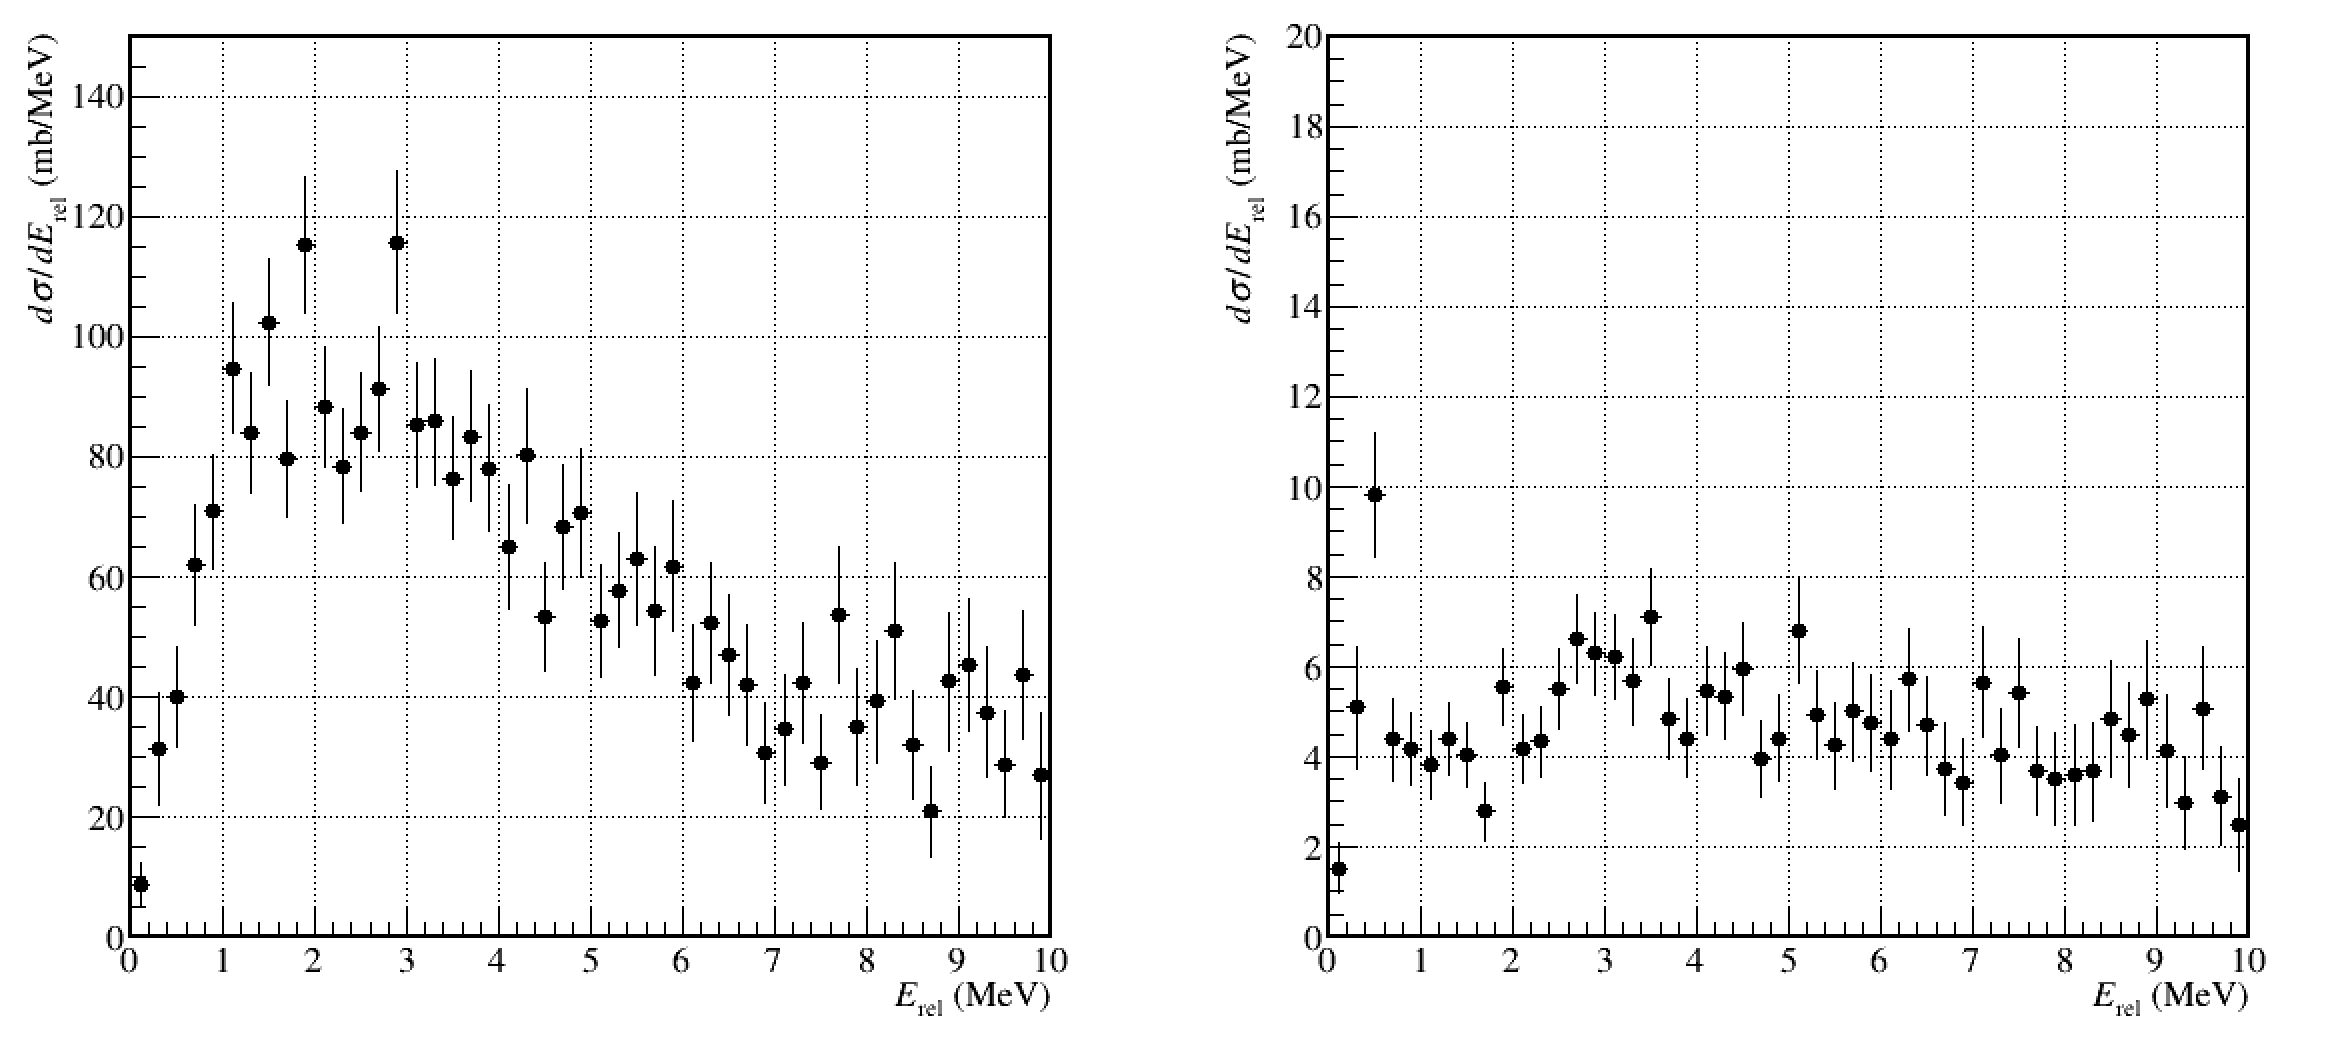
\includegraphics[width=\textwidth]{chapter4/sigma_fnn.png}
    \caption{Differential cross section of ${}^{15}\text{B} + n + n$ for Pb target (left) and C target (right)}
    \label{fig:sigma_fnn}
\end{figure}
\begin{figure}
    \centering
    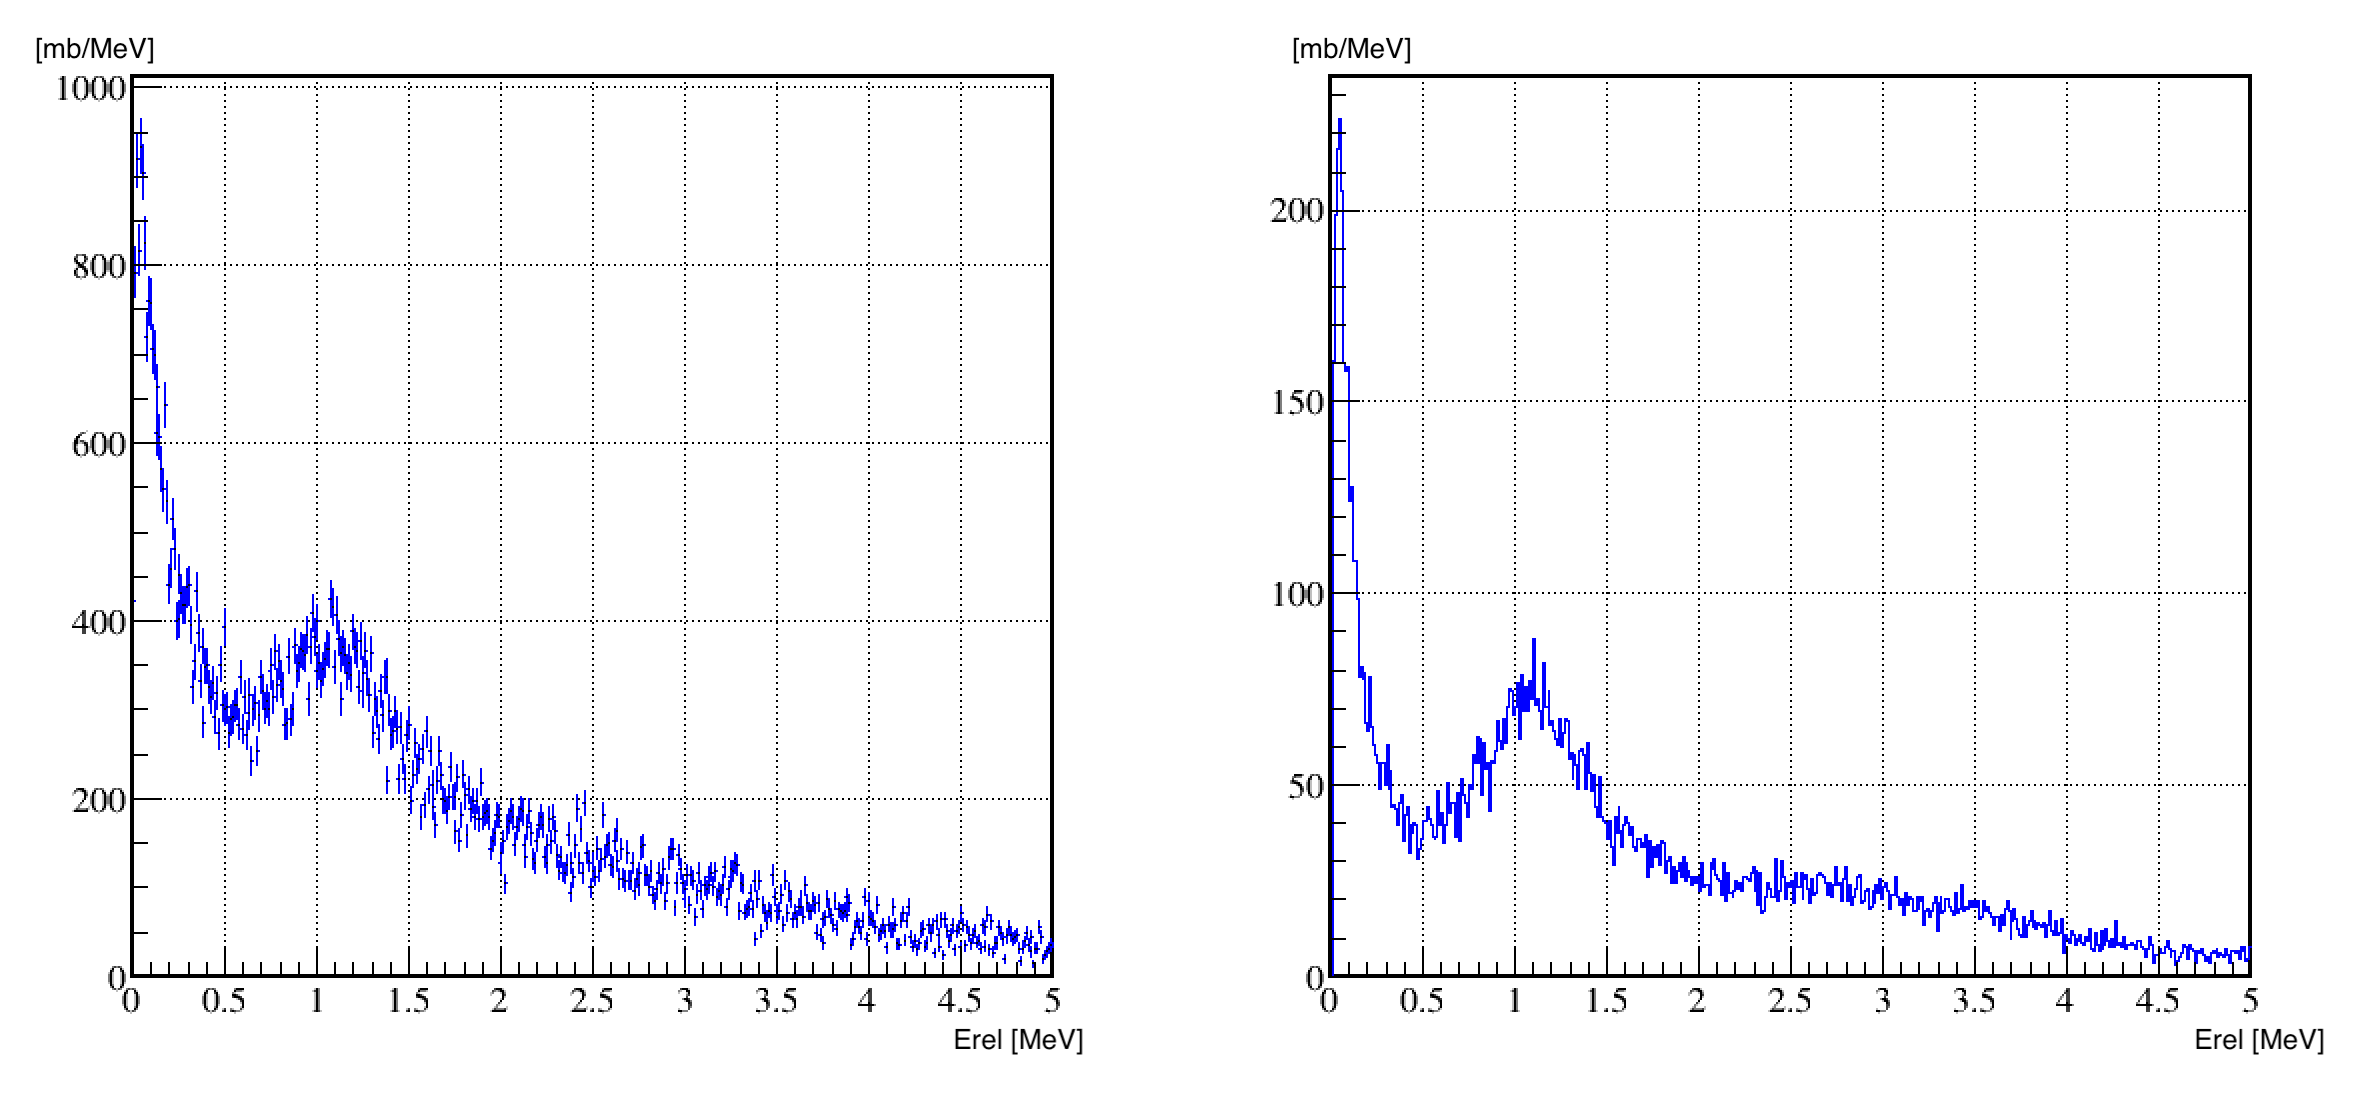
\includegraphics[width=\textwidth]{chapter4/sigma_fn.png}
    \caption{Differential cross section of ${}^{15}\text{B} + n$ at Pb target (left) and C target (right)}
    \label{fig:sigma_fn}
\end{figure}
